
\documentclass[a4paper,oneside,12pt]{article}

\usepackage[utf8]{inputenc}    % make čšž work on input
\usepackage[T1]{fontenc}       % make čšž work on output
\usepackage[slovene]{babel}    % slovenian language and hyphenation
\usepackage[reqno]{amsmath}    % basic math
\usepackage{amssymb,amsthm}    % math symbols and theorem environments
\usepackage{graphicx}          % images
\usepackage{enumerate}
\usepackage{subcaption}
\usepackage{graphicx}
\usepackage[
  paper=a4paper,
  top=2.5cm,
  bottom=2.5cm,
  left=2.5cm,
  right=2.5cm
% textheight=24cm,
]{geometry}  % page geomerty

% vstavi svoje pakete tukaj
\usepackage{fancyhdr}
\usepackage{harpoon}
\usepackage{tikz}
\usepackage{makeidx}
\makeindex
\usepackage[all]{xy}
\usepackage{minted}
  % algorithms
  % \RequirePackage{algpseudocode}  % za psevdokodo
  % \RequirePackage{algorithm}      % za plovke
  % \floatname{algorithm}{Algoritem}
  % \renewcommand{\listalgorithmname}{Kazalo algoritmov}



% clickable references, pdf toc
\usepackage[bookmarks, colorlinks=true, linkcolor=black, anchorcolor=black,
  citecolor=black, filecolor=black, menucolor=black, runcolor=black,
  urlcolor=black, pdfencoding=unicode]{hyperref}



% stavi lastne definicije tukaj
% \newcommand{\dpar}[2]{\frac{\partial #1}{\partial #2}}
% \newcommand{\HH}{$\mathcal{H}$}
% \newcommand{\LL}{$\vec{\ell}$}
% \newcommand{\AA}{$\vec{{A}}$}
  % \floatname{listing}{Koda}
  % \renewcommand{\listalgorithmname}{Kazalo programske kode}
% \pagestyle{empty}              % vse strani prazne (ni okraskov, številčenja....)
 \setlength{\parindent}{0pt}    % zamik vsakega odstavka
% \setlength{\parskip}{10pt}     % prazen prostor pod odstavkom
%\setlength{\overfullrule}{30pt}  % oznaci predlogo vrstico z veliko črnine
\frenchspacing % to se priporoča, da bo presledek za piko na koncu stavka enako dolg kot obični.
%Alternativa je ročno metanje \ za vsako okrajšavo.
\usepackage{braket}
\usepackage{todonotes}
\hypersetup{pdftitle={201: Navadne diferencialne enačbe: začetni problemi}, pdfauthor={Peter Rupnik}} %To piše v pdf viewerju na vrhu! veri neat
\title{201: Navadne diferencialne enačbe: začetni problemi}
\author{Peter Rupnik}
\begin{document}
\maketitle
\section{Naloga}
\begin{enumerate}

\item S pomočjo podprogramov za metodo Runge-Kutta zasleduj gibanje
  planeta na tiru okrog sonca. Opazuj stabilnost razdalje obeh teles
  pri krožnem gibanju. Preveri točnost obhodnega časa ter  
  natančnost povratka pri eliptičnih tirih, zlasti pri tistih z majhno
  začetno hitrostjo. Opazuj stalnost energije in vrtilne količine.

\item Razišči obnašanje planeta v krožni orbiti,
  če sonce nadomestite s parom polovičnih sonc,
  v odvisnosti od njune medsebojne razdalje.
  Sonci sta v krožni orbiti okrog skupnega težišča, vpliv planeta na njuno
  orbito zanemarimo.

\item Trk zvezde in planetnega sistema: mimo sonca s planetom na
  krožnem tiru pridrvi v tirni ravnini druga zvezda z enako
  maso. Mimobežna zvezda vpada s hitrostjo, ki je enaka dvakratni
  obodni hitrosti planeta in potuje po ravni črti v razdalji 1.5
  radija planetnega tira (nalogo smo poenostavili z zanemaritvijo
  keplerskega tira prihajajoče zvezde).  Razišči končno usodo planeta
  v odvisnosti od njegove faze. Račun začnemo, ko je vpadna zvezda še
  10 radijev planetnega tira daleč od svojega perihelija in ga
  končamo, ko se znajde v točki, ki je simetrična na začetno. Kaj se
  spremeni, če smer gibanja planeta obrnemo?

  
\end{enumerate}

\section{Reševanje}
\subsection{Podnaloga 1}
Najprej se uverim, da lahko iz začetnih pogojev pravilno integriram časovni razvoj. Izbral sem si nekaj začetnih hitrosti, za katere vemo, kakšne orbite porodijo. Za orbite\footnote{brez upoštevanja simetrije $v_0 \rightarrow - v_0$  in izrojenih elips za $v_0 = 0$} velja:
\[
    \mathrm{orbita}=\begin{cases}
        \mathrm{kro\check{z}nica}, & v_0 = 1,        \\
        \mathrm{hiperbola},        & v_0 = \sqrt{2}, \\
        \mathrm{parabola},         & v_0 > \sqrt{2}, \\
        \mathrm{elipsa},           & \mathrm{sicer}
    \end{cases}
\]

Za \(v_0 \in \left{ 1, \sqrt{2}, 1.5, 0.5, 0.3 \right}\) sem izračunal trajektorije v časovnem intervalu $ t\in\left[ 0, 10\right] $ z adaptivnim časovnim korakom z metodo \texttt{scipy.integrate.solve\_ivp}.

\begin{center}
    \centering
    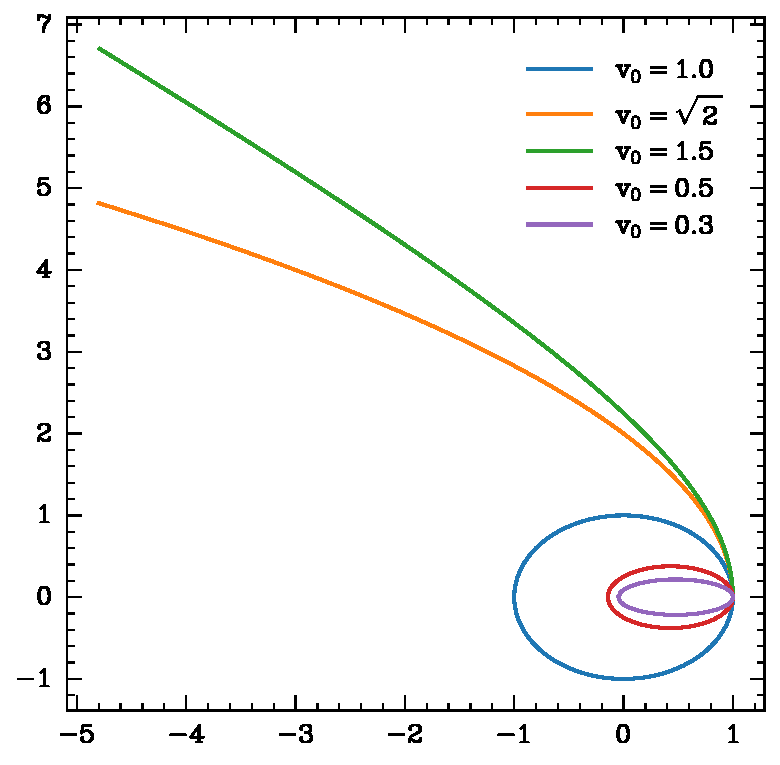
\includegraphics[width=0.5\textwidth]{../images/1-1-v0.pdf}
\end{center}

Naslednji korak je študija invariantnih količin. Zanimalo nas bo spreminjanje polne energije $H$, vrtilne količine $\mathbf{L}$,  in Laplace-Runge-Lenzovega vektorja $\mathbf{A}$ skozi čas za različne začetne pogoje. Rezultate prikazujem na sliki~\ref{fig:1-1-energija}.

\begin{figure}
    \label{fig:1-1-energija}
    \centering
    \begin{subfigure}{0.49\textwidth}
        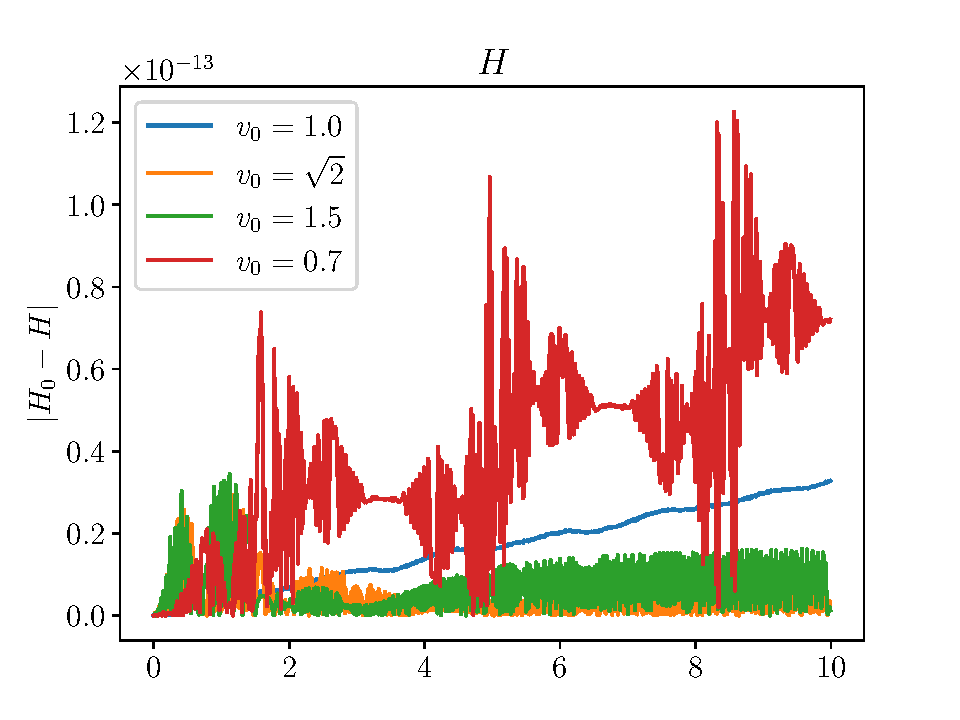
\includegraphics[width=\textwidth]{../images/1-1-H_lin.pdf}
    \end{subfigure}
    \hfill
    \begin{subfigure}{0.49\textwidth}
        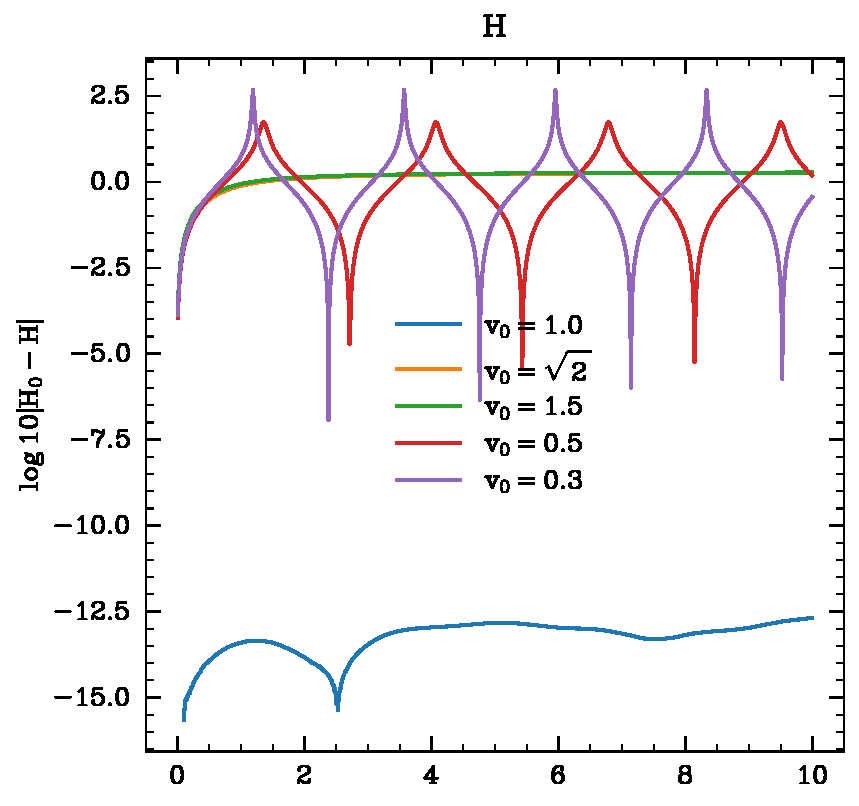
\includegraphics[width=\textwidth]{../images/1-1-H_log.pdf}
    \end{subfigure}
    \newline
    \begin{subfigure}{0.49\textwidth}
        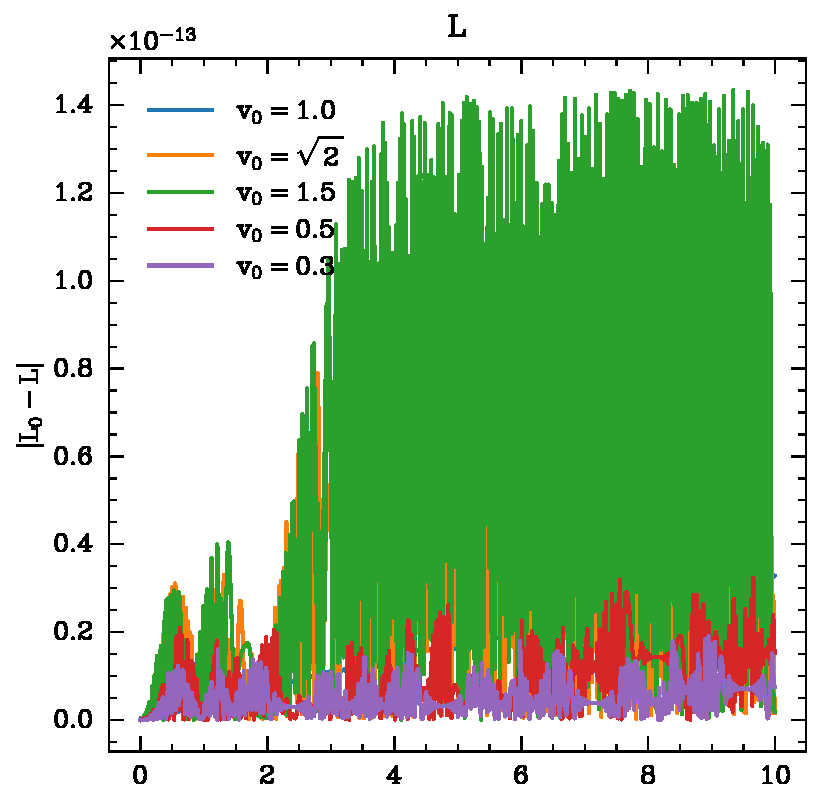
\includegraphics[width=\textwidth]{../images/1-1-L_lin.pdf}
    \end{subfigure}
    \hfill
    \begin{subfigure}{0.49\textwidth}
        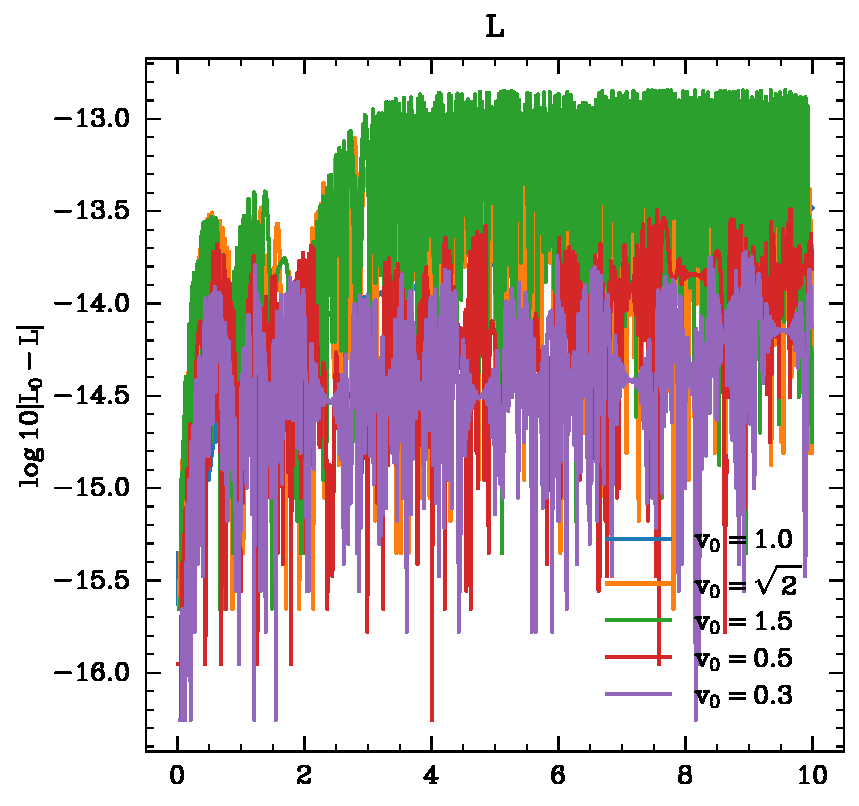
\includegraphics[width=\textwidth]{../images/1-1-L_log.pdf}
    \end{subfigure}
    \newline

    \begin{subfigure}{0.49\textwidth}
        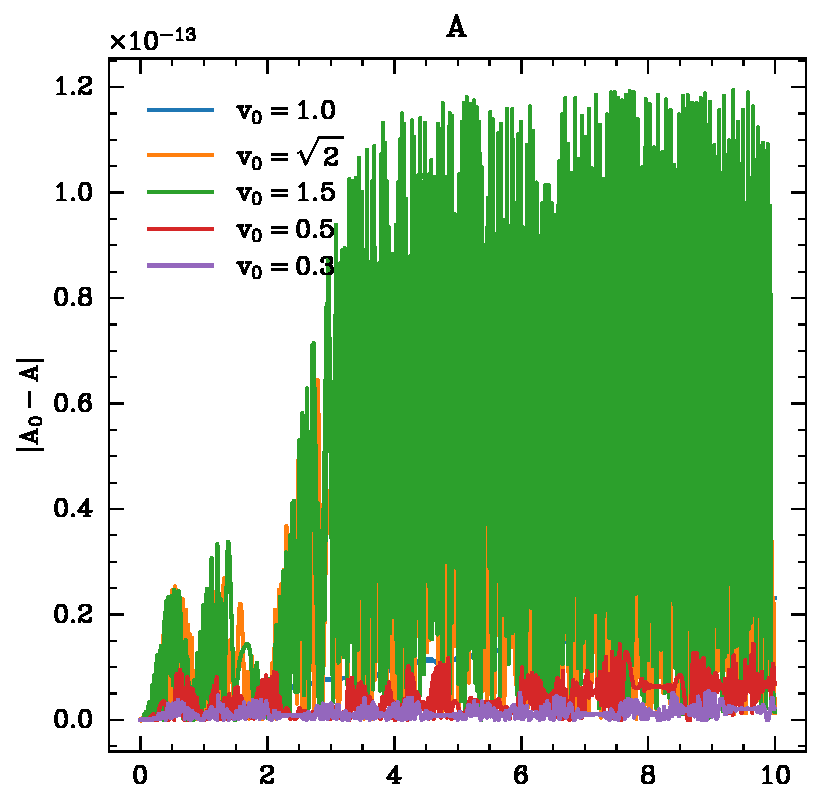
\includegraphics[width=\textwidth]{../images/1-1-A_lin.pdf}
    \end{subfigure}
    \hfill
    \begin{subfigure}{0.49\textwidth}
        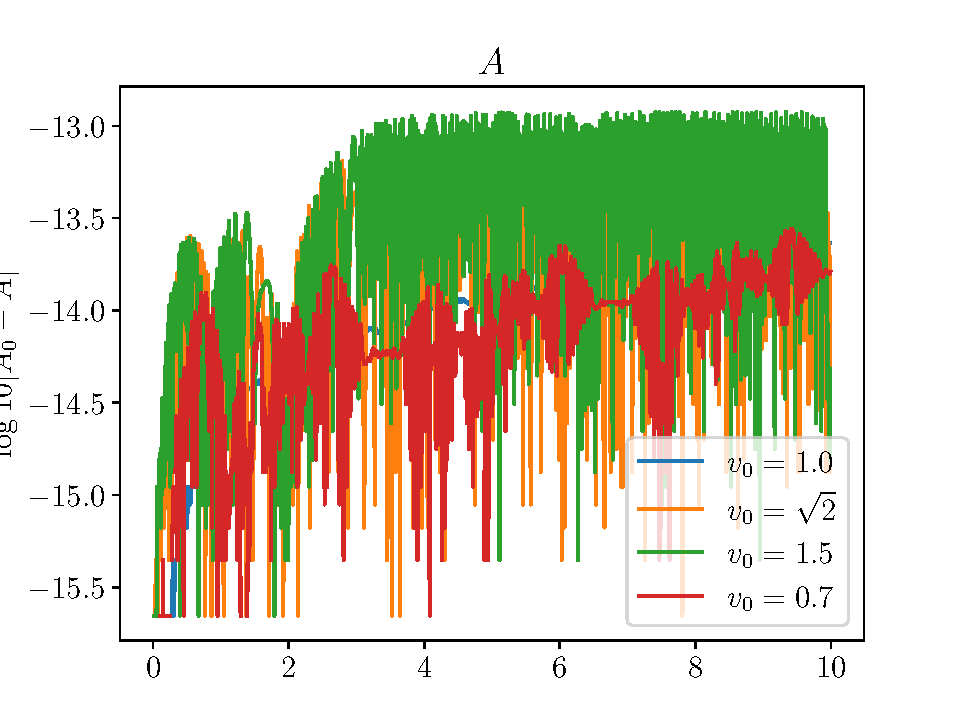
\includegraphics[width=\textwidth]{../images/1-1-A_log.pdf}
    \end{subfigure}
    \caption{Časovni poteki invariantnih količin. V vseh primerih se količine najlepše obnašajo za krožno orbito. Polna energija $H$ je najbolj nestabilna.}

\end{figure}

Za študijo stabilnosti obhodnih časov sem implementiral \texttt{event tracker}, funkcijo, katere koren bo integrator iskal. Pri tem sem se posvetil primerom, ko $v_0<\sqrt{2}$, da zagotovim periodičnost orbit. Uporabljena je bila sledeča metodologija: za vsak $v_0$ sem iskal orbito za $t\in \left(0, 21\pi \right)$, pri čemer mi je prehode čez $y=0$ iskal integrator sam.  Dobljene čase prehoda sem numerično odvajal, da dobim čase med zaporednimi prehodi, nato pa sem izračunal povprečno periodo in standardno deviacijo. Rezultate prikazujem na naslednji sliki.


\begin{center}
    \centering
    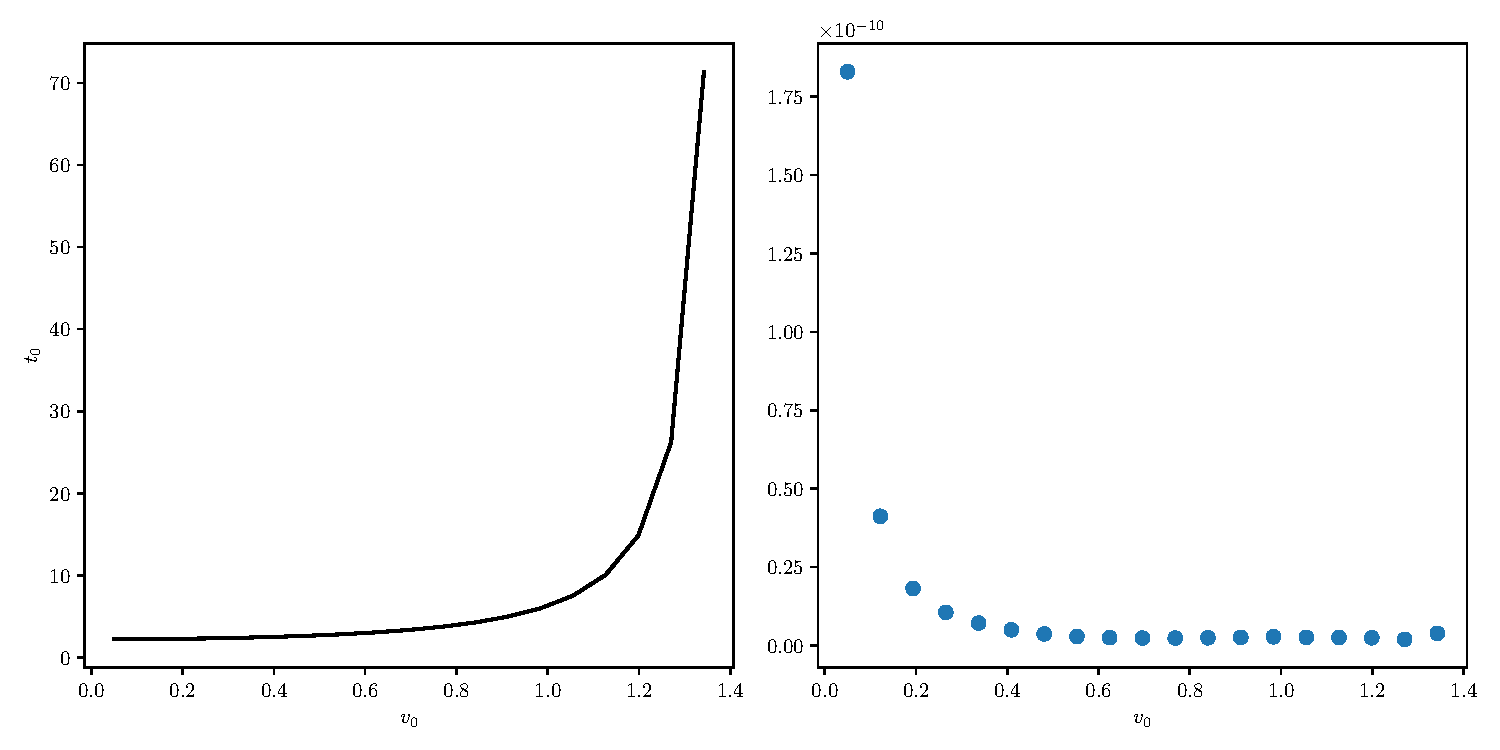
\includegraphics[width=0.9\textwidth]{../images/1-2-t0.pdf}
    {Stabilnost obhodnega časa. [Levo] povprečne vrednosti zaporednih obhodnih časov s standardnimi deviacijami. [Desno] standardne deviacije intervalov med zaporednimi prehodi.}
    % \label{fig:1-2-t0}
\end{center}

Pri nizkih začetnih hitrostih standardna deviacija zaporednih izmerkov strmo naraste, kar lahko pripišemo težavam, na katere naleti integrator v bližini pola potenciala.
\subsection{Podnaloga 2}

Nato sem popravil cevovod za integracijo tako, da je upošteval prispevek dveh pol-sonc, ki krožita okrog skupnega težišča z nastavljivo kotno hitrostjo, nastavljivo medsebojno razdaljo, in nastavljivim zamikom glede na planet.

Raziskal sem, kakšne orbite lahko dobim z različnimi nastavitvami začetnih parametrov. Z rumeno prikazujem orbiti sonc.
\begin{center}
    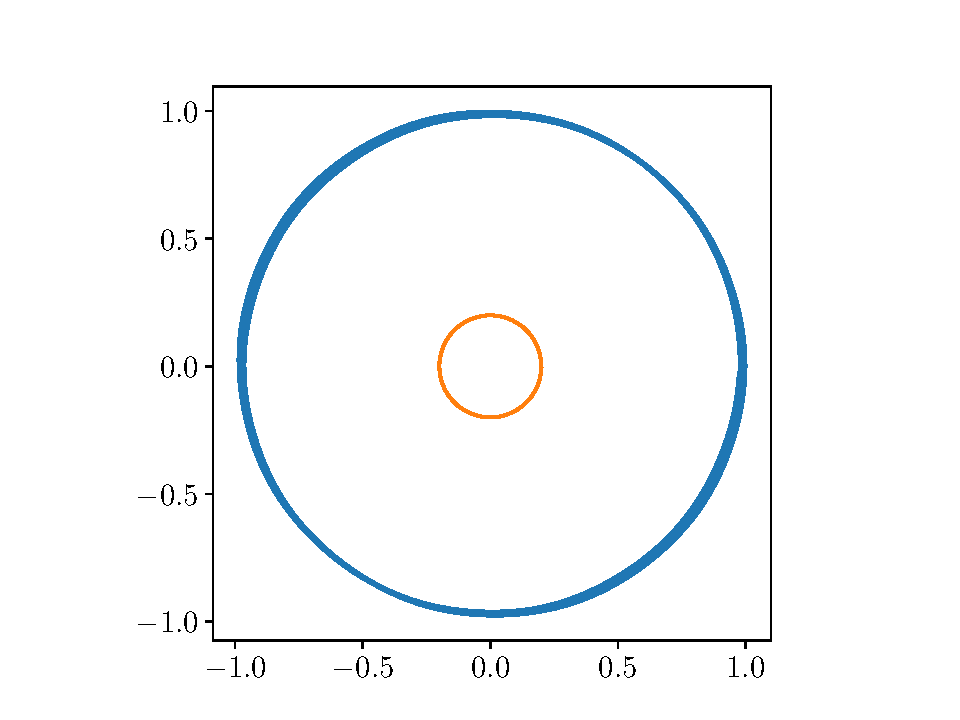
\includegraphics[width=0.5\textwidth]{../images/2-1-orbite_1.pdf}\hfill
    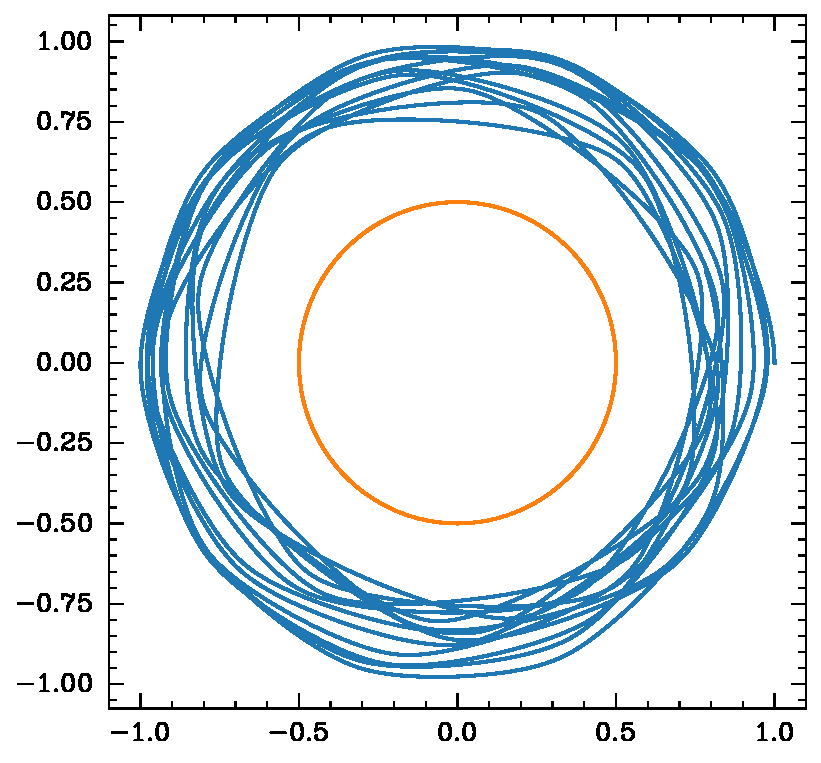
\includegraphics[width=0.5\textwidth]{../images/2-1-orbite_2.pdf}

    % \includegraphics[width=0.5\textwidth]{../images/2-1-orbite_3.pdf}\hfill
    % \includegraphics[width=0.5\textwidth]{../images/2-1-orbite_4.pdf}
\end{center}

Za študijo vpliva dvozvezdja na dinamiko planeta pogledam krožne orbite planeta pri $v_0 = 1$. Z variacijo razdalje med polsoncema~$r$ opazujem, kaj se dogaja s povprečjem in standardno deviacijo oddaljenosti  orbite planeta od masnega središča sistema. V analizo sem vključil samo primere, kjer planet ne 'pobegne'. Kotna hitrost polsonc je v vseh poskusih znašala $2\pi$. Trajektorije sem integriral do časa $t=60$, začetna hitrost planeta je bila fiksirana na $v_0=1$.

Kot pričakovano je vpliv večji pri večjih medzvezdnih razdaljah, ko $r \rightarrow d$, viden pa je že pri majhnih. Presenetljivo je vpliv dvozvezdja bolj opazen, ko je ob času~0 zveznica med polsoncema navpična.

\begin{center}
    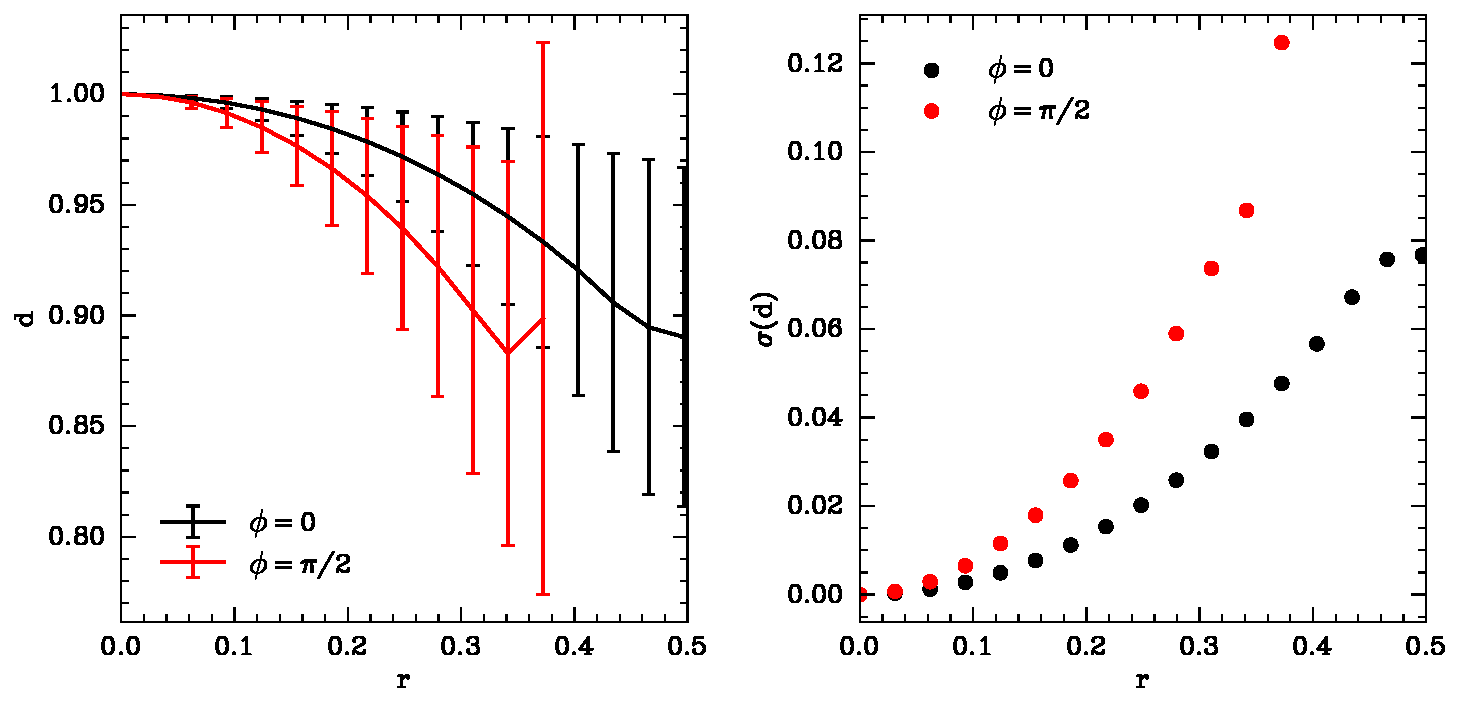
\includegraphics[width=0.9\textwidth]{../images/2-2-vplivr.pdf}
\end{center}
\subsection{Podnaloga 3}

Za študijo preleta mimobežne zvezde sem spet pripravil cevovod za integracijo. Tokrat sem poleg koordinat in impulzov planeta integriral še vodoravno koordinato mimobežne zvezde, kar sem lahko uporabil kot signal za končanje terminacije (kot opisano v prvi podnalogi.) Za začetne pogoje vzamem
\[
    y_0 =
    \begin{bmatrix}
        x \\
        y \\
        v \\
        u \\
        x_2
    \end{bmatrix} =
    \begin{bmatrix}
        \cos{\phi}       \\
        \sin{\phi}       \\
        - v_0 \sin{\phi} \\
        v_0 \cos{\phi}    \\
        -10
    \end{bmatrix},
\]

kjer je $x_2$ vodoravna koordinata mimobežne zvezde. Parametra $\phi$ in $v_0$ si pustim prosta za eksperimentacijo. Za boljši uvid integracijo pustim teči dlje kot naloga zahteva, nato pa po izračunanih trajektorijah izračunam energije $H$, $H_1$, in $H_2$, definirane kot:
\begin{align*}
T &= \frac{u^2 +v^2}{2},\nonumber \\
d_1 &= \sqrt{(x - 0)^2 + (y - 0)^2}\nonumber \\
d_2 &= \sqrt{(x - x_2)^2 + (y - 1.5)^2}\nonumber \\
H &= T - \frac{1}{d_1} - \frac{1}{d_2}\nonumber \\
H_1 &= T - \frac{1}{d_1}\nonumber \\
H_2 &= T - \frac{1}{d_2} \nonumber
\end{align*}

S preletom parametrskega prostora lahko najdem nekaj zanimivih primerov, kjer mimoleteče sonce spremeni orbito planeta, s svojim gravitacijskim privlakom izbije planet iz prvotne orbite, ali pa potegne planet za seboj. Želel sem prečesati prostor parametrov $v_0$ in $\phi$ in s pomočjo značilk $H$, $H_1$, $H_2$ avtomatsko določiti usodo planeta, a na podlagi ročnega opazovanja ne opazim dobre hevristike.

\begin{center}
    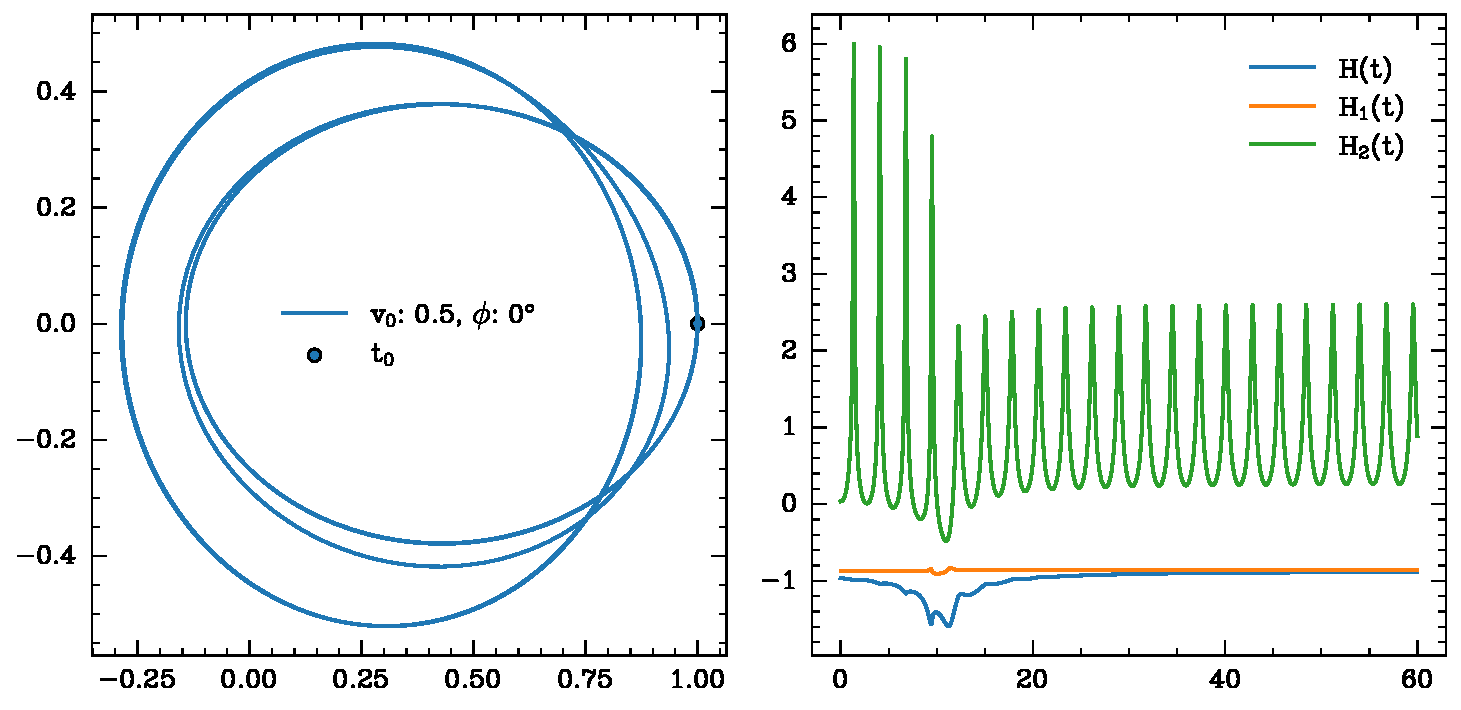
\includegraphics[width=0.9\textwidth]{../images/3-1-0.pdf}
\end{center}
\begin{center}
    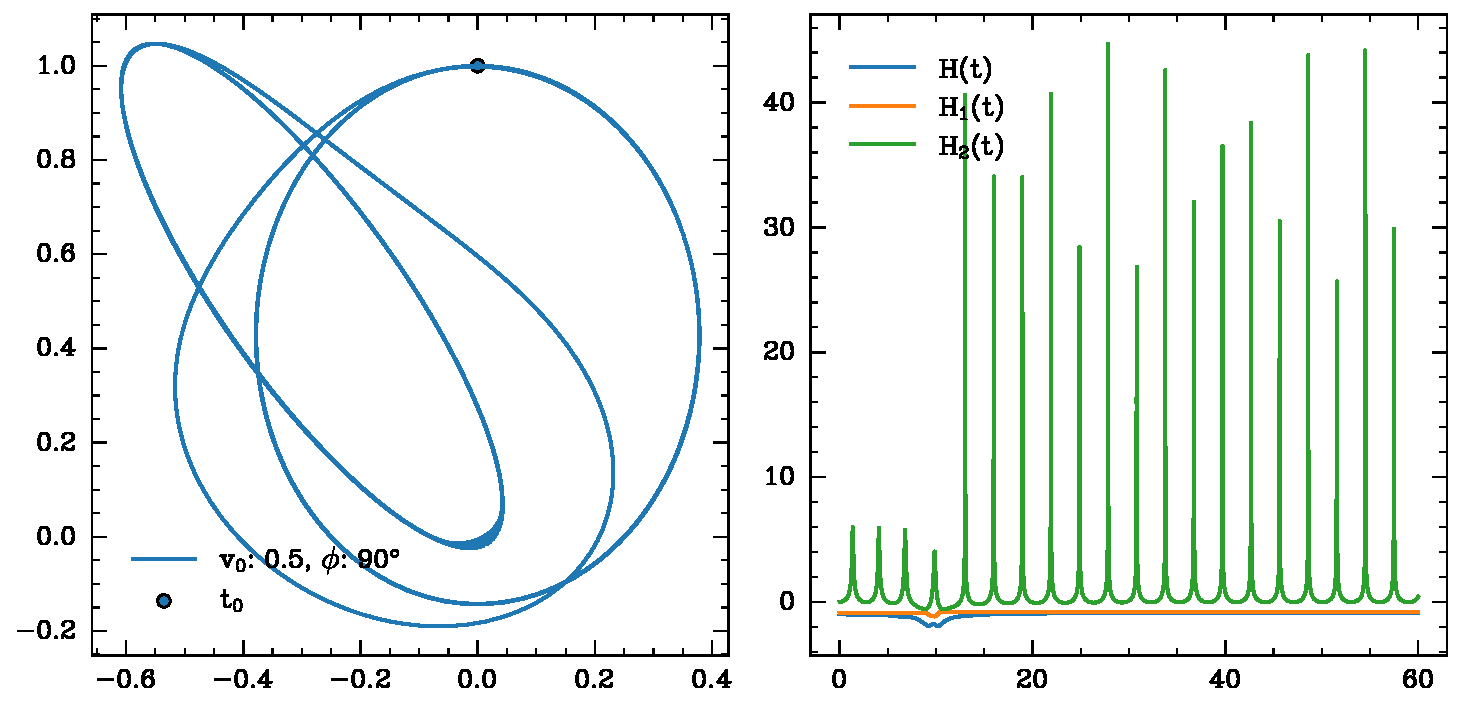
\includegraphics[width=0.9\textwidth]{../images/3-1-2.pdf}
\end{center}

\begin{center}
    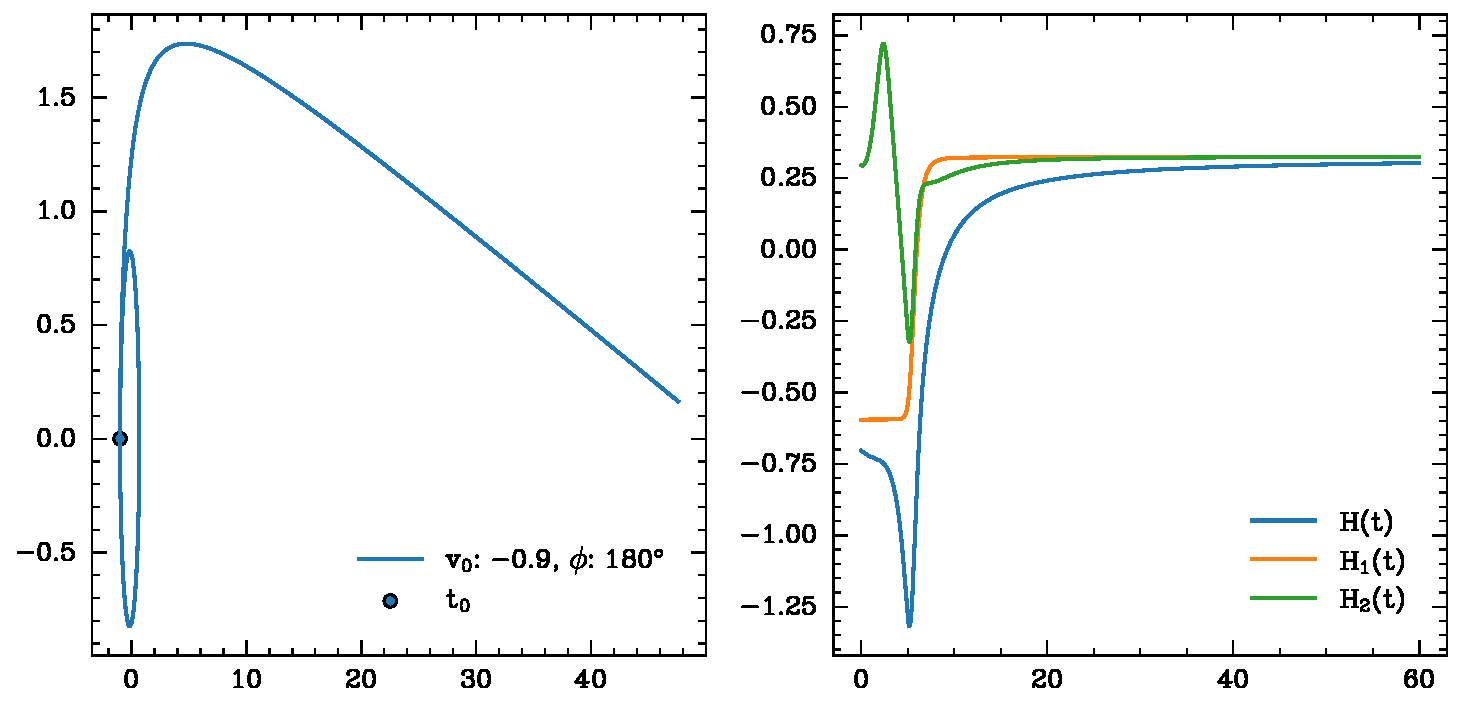
\includegraphics[width=0.9\textwidth]{../images/3-1-60.pdf}
\end{center}
\begin{center}
    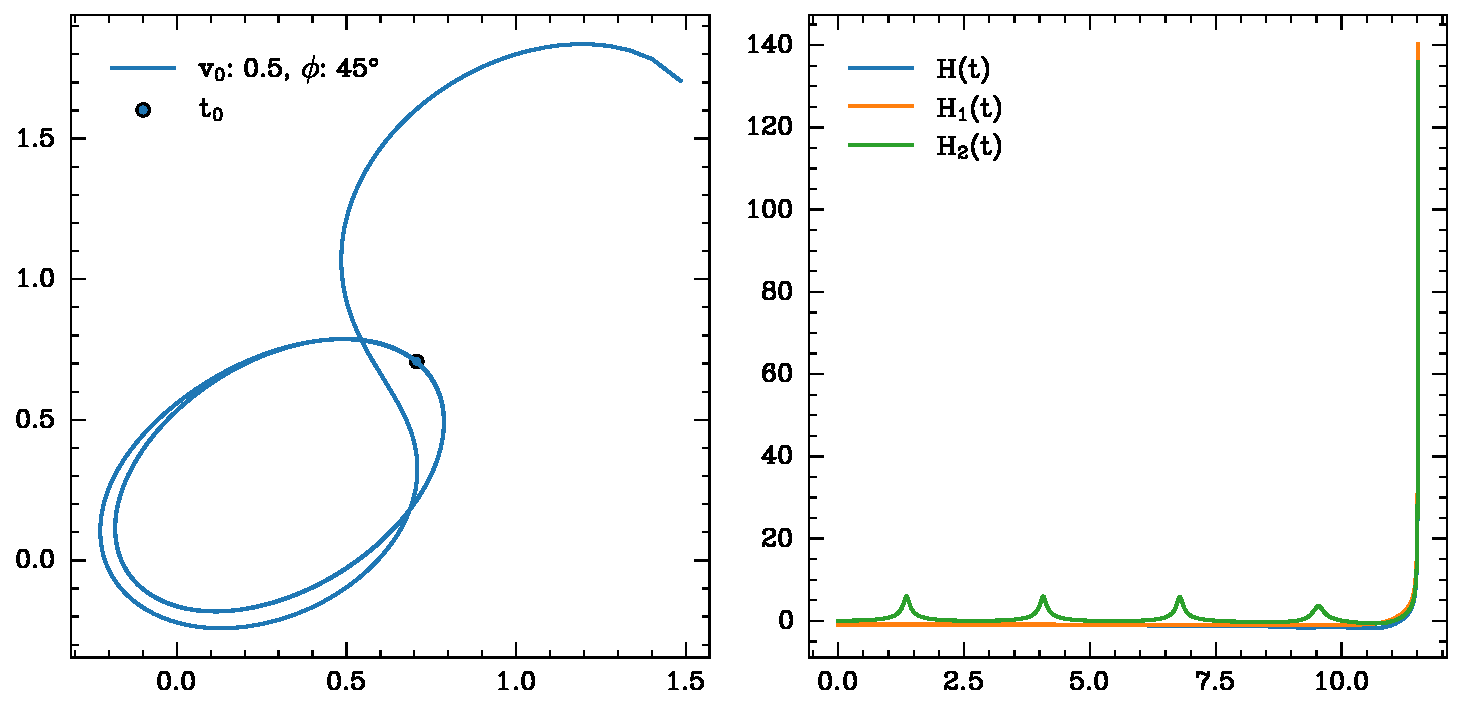
\includegraphics[width=0.9\textwidth]{../images/3-1-1.pdf}
\end{center}


\end{document}

\begin{center}
     \includegraphics[width=0.7\textwidth]{}
\end{center}
\begin{figure}
    \centering
        \begin{minipage}{0.45\textwidth}
        \centering
    \includegraphics[width=\textwidth]{}
    \caption{} 
        \label{fig:}
    \end{minipage}\hfill
    \begin{minipage}{0.45\textwidth}
        \centering
        \includegraphics[width=1\textwidth]{}
    \caption{}
    \label{fig:}
    \end{minipage}
\end{figure}
\begin{figure}
    \centering
    \includegraphics[width=0.9\textwidth]{}
    \caption{Caption}
    \label{fig:my_label}
\end{figure}